\section{Discussion}
\label{sec:disc}


\newcommand{\allp}{\texttt{all\_p}}
\newcommand{\onp}{\texttt{on\_p}}
\newcommand{\offp}{\texttt{off\_p}}
\newcommand{\hystp}{\texttt{hyst\_p}}
\newcommand{\aonebelow}{\texttt{a1\_below}}
\newcommand{\atwobelow}{\texttt{a2\_below}}
\newcommand{\aoneabove}{\texttt{a1\_above}}
\newcommand{\atwoabove}{\texttt{a2\_above}}
\newcommand{\doion}{\texttt{doi\_on}}
\newcommand{\done}{\texttt{d1}}
\newcommand{\dtwo}{\texttt{d2}}
\newcommand{\abovehyst}{\texttt{above\_hyst}}
\newcommand{\inhibit}{\texttt{inhibit}}

In this section we show how traceability and coverage analyses can be performed using IVCs.
The goal of this section is to both illustrate the techniques and discuss the potential pitfalls of the analysis. Here we adapt the same ASW example presented in Section \ref{sec:example}. The code is slightly changed so we can discuss how IVCs help to improve the design and specification.

% \begin{figure}[t]
%\centering
%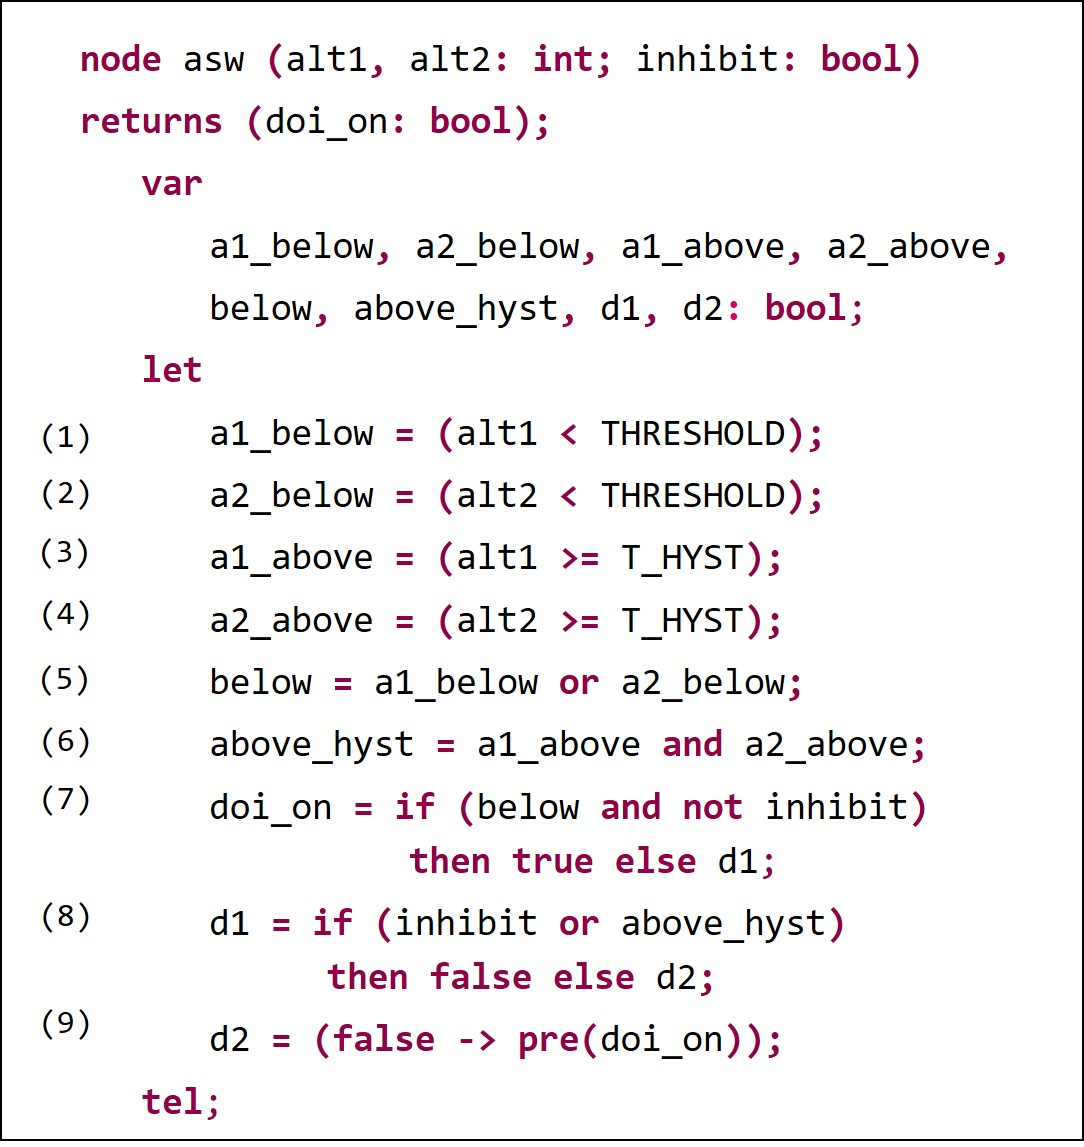
\includegraphics[width=0.9\columnwidth]{figs/code.jpg}
%\vspace{-0.1in}
%\caption{Altitude Switch Model}
%\vspace{-0.1in}
%\label{fig:asw2}
%\end{figure}

 We illustrate the results with traceability matrices produced by the  \texttt{Spear} requirements specification tool~\cite{Spear}.  \texttt{JKind} is used as the model checker for the  \texttt{AADL AGREE} tool suite~\cite{NFM2012:CoGaMiWhLaLu} and also \texttt{Spear} ~\cite{Spear}.  We have extended both tools to add graphical support for displaying adequacy and traceability results.  We show screenshots for the  \texttt{Spear} tool for our running example in Figures~\ref{fig:propertyset1} and~\ref{fig:propertyset4}.

The ASW is responsible for turning on and off a device of interest, so we formulate two requirements that describe when the ASW should be {\em on} and when it should be {\em off}.  The first attempt at formalization (property set 1) is as follows:

%\begin{definition} {\emph{ASW Requirements Version 1} }
{\smaller
\begin{verbatim}
on_p = (a1_below and a2_below) and not inhibit =>
    doi_on = true;
off_p = (a1_above and a2_above) and inhibit =>
    doi_on = false;
all_p = on_p and off_p;
\end{verbatim}
}
%\end{definition}

\begin{figure}
  \centering
  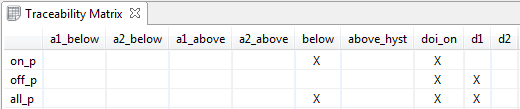
\includegraphics[width=\columnwidth]{figs/spear_set1.png}
  \vspace{-0.1in}
  \caption{Elements covered by the initial property set}
  \vspace{-0.1in}
  \label{fig:propertyset1}
\end{figure}


\noindent Informally, when both altimeters are below the threshold and not inhibited, then the DOI should be on (\onp), and when both altimeters are below the threshold and the ASW is inhibited, then the DOI should be off (\offp).
For each of the \ivccov, \maycov, and \mustcov\ metrics, \allp\ only requires \texttt{\{below, d1, doi\_on\}}, as shown in Figure~\ref{fig:propertyset1}.   This small set of elements is due to a classic specification problem: using computed variables as the antecedents of implications.  If these values are computed incorrectly (say, we choose the wrong threshold for \aonebelow), it may cause the property to be valid for incorrect reasons.

%This is alarming, and somewhat puzzling, because one would think that at least the definitions of the `below' or `above' would be necessary.  However, because the specification used the model variables \aonebelow, \atwobelow, \aoneabove, and \atwoabove, the actual valuations of the thresholds do not matter.  This situation illustrates a classic specification problem: using computed variables in the antecedents of implications.
%\footnote{\noindent ~In this case, if the computation of the variables used in the antecedent is incorrect, then our property will not verify what it is expected to verify \mike{citation to one of our papers on specification here...}; note also that this does not mean the property is necessarily {\em vacuous}.}

We therefore modify our properties to use inputs and constants as antecedents and derive:

{\smaller
\begin{verbatim}
on_p = ((alt1 < THRESHOLD) and (alt2 < THRESHOLD))
   and not inhibit => doi_on = true;
off_p = ((alt1 >= T_HYST) and (alt2 >= T_HYST))
   and inhibit => doi_on = false;
\end{verbatim}
}
% all_p = on_p and off_p;
%\end{definition}

\noindent In this version, distinctions emerge between the metrics.  \allp\ has two \mivc s: \texttt{\{\{a1\_below, below, doi\_on, d1\}, \{a2\_below, below, doi\_on, d1\}\}}, because of the \onp\ property: in the implementation, the DOI is turned on when either of the altimeters is below the threshold, while our property states that they both must be below.
Domain experts determine that the requirement is correctly specified and that our implementation is a reasonable refinement, so there is no need to change the model or the property.  The MUST elements are the same as version 1: \texttt{\{below, doi\_on, d1\}}, because neither \aonebelow\ or \atwobelow\ is required for all proofs.  %However, given the MUST elements, we can no longer construct a proof, because at one of these definitions is necessary for either proof.
The MAY elements contain both \aonebelow\ and \atwobelow.

The \abovehyst, \aoneabove, \atwoabove, and \dtwo\ equations are still missing, meaning that the ``above'' thresholds are irrelevant to our properties.  Examining \offp, we realize that we have a specification error; the DOI should be off if either \inhibit\ is true or both altimeters are above the threshold. The fix is:

%\begin{definition} {\emph{ASW Requirements Version 2} }
{\smaller
\begin{verbatim}
off_p = ((alt1 >= T_HYST) and (alt2 >= T_HYST))
   or inhibit => doi_on = false;
\end{verbatim}
}
%on_p = ((alt1 < THRESHOLD) and (alt2 < THRESHOLD))
%   and not inhibit => doi_on = true;
%all_p = on_p and off_p;
%\end{definition}

\noindent Now the \allp\ requirement proof yields a single \mivc ~that requires all variables except \{\texttt{d2}\}, so \mivc ~= MAY = MUST.  Interestingly, the \offp\ proof requires both the lower altimeter thresholds even though the \onp\ proof does not; the reason is that if either of these is false, then \doion\ will be true.  To cover \{\texttt{d2}\}, we realize no property covers the hysteresis case, so an additional property is added for this case:

%\begin{definition} {\emph{ASW Requirements Version 2} }
{\smaller
\begin{verbatim}
hyst_p = not inhibit and
         (alt1 > THRESHOLD and alt2 > THRESHOLD) and
         (alt1 < T_HYST or alt2 < T_HYST) =>
   (doi_on = false -> doi_on = pre(doi_on))
all_p = on_p and off_p and hyst_p;
\end{verbatim}
}
%on_p = ((alt1 < THRESHOLD) and (alt2 < THRESHOLD))
%   and not inhibit => doi_on = true;
%all_p = on_p and off_p;
%\end{definition}
\noindent The final property states that if the antecedent conditions hold, then in the initial state, the \doion\ variable is assigned false, and in subsequent steps, it retains the same value as it previously had.

\begin{figure}
  \centering
  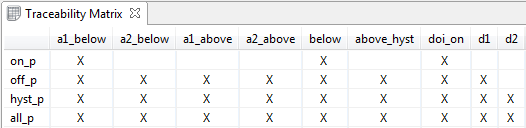
\includegraphics[width=\columnwidth]{figs/spear_set4.png}
  \vspace{-0.1in}
  \caption{Elements covered by the final property set}
  \vspace{-0.1in}
  \label{fig:propertyset4}
\end{figure}

As shown in Figure~\ref{fig:propertyset4}, the measures again coincide and include all variables, and we appear to have a reasonably complete specification.  However, the measures are certainly not foolproof; it turns out that using {\em only} the hysteresis property \hystp\ will {\em also} yield a ``complete'' result for all of the metrics: to establish its validity, all of the equations that we have defined in the model are required.  This is because the partitioning of the transition system (i.e., the equations) is insufficiently {\em granular} to detect the incompleteness.
%However, this one property would not reasonably be considered a complete specification.
%We will examine this situation further in the discussion section~\mike{add this!}.
%
%\mike{How would we define a metric that would flag the model as incomplete?  Model transformation would do it: if we added separate variables for each assignment of doi\_on, then any of the metrics would flag the \hystp\ spec as incomplete.}

\iffalse As mentioned, IVCs are derived from inductive invariants; in other words, they are built upon the proof of the validity of a given property. One interesting fact about proofs
  is that a given property could be proved from different proof paths.
  The $AIVC$ captures this fact and gives a clear picture of various ways a property is satisfied. By getting all the MIVCs for the system properties and categorizing them, one can find if there are design artifacts that do not trace to any property: set $\bigcap \{IRR (P) | P \in \Delta \}$.  If this set is non-empty, it is a possible indication of ``gold plating" or missing properties \cite{Murugesan16:renext}.
\fi

\subsection{Granularity}

As we described in Section \ref{sec:background}, transition relation is considered
as the conjunction of Boolean formulas. The granularity of these formulas substantially affects the analysis results.  In the presented example, it was possible to have a ``complete'' specification of the model involving only the hysteresis property \hystp.  The way that the model was structured, in order to determine the validity of the property, all of the equations in the model were required.  However, for this property certain subexpressions of the equations were irrelevant, notably the value assigned to the \texttt{doi\_on} variable in the \texttt{then} branches of equations (7) and (8).  If we decompose the equations into smaller pieces, e.g., creating separate equations for the \texttt{then} and \texttt{else} branches, this incompleteness becomes visible and the model is no longer completely covered.


%\mike{Oy...this section needs improvement}

%Splitting a model into more conjuncts will make coverage scores more accurate and usually lower, though it will not always lower coverage scores.
%
We have explored granularity within the context of the Lustre language.  Lustre provides a nice formalism for discussion because it is top-level conjunctive (as required by our IVC definition), equational, and {\em referentially transparent}: the behavior of a Lustre program is defined by a system of equations, and any subexpression on the right side of an equation can be extracted and assigned to a ``fresh'' variable which is substituted into the original equation without changing the meaning of a program.  In this context, we can define a {\em granular refinement} as an extraction of a subexpression into a fresh equation involving a ``fresh'' variable.

We call a Lustre model {\em sufficiently granular} if each computed (i.e., non-input) variable is used at most once in the right-hand side of an equation, and each equation is either a single operator (which may be a ternary operator in the case of if-then-else) with leaves all variable expressions, or a constant expression.  Intuitively, one can think of a model meeting this criteria as completely decomposed, where each instance of a subexpression in the original model is assigned its own variable.  

If a set of requirements achieves 100\% coverage of a sufficiently granular model, then no granular refinement will achieve less than 100\% coverage.  This is straightforward to show in a proof sketch.  Based on the right side of the equation, there are two cases: (1) the entire right-hand side of the equation is extracted (which may be a constant or a single operator expression). In this case, by assumption the variable assigned is necessary for proof, so its definition must be necessary for the proof; in this case, the ``fresh'' variable must also be necessary for the proof; (2) a ``leaf'' expression of the single right-hand side operator is extracted.  Since (by definition) the leaf is a variable expression that is used only once, and (by assumption) the variable is necessary for proof, then the ``fresh'' variable is also necessary for proof.

We have implemented a transformation that splits models into {\em sufficiently granular} conjuncts.  In a small initial experiment involving 30 of the original models, we performed our transformation and re-ran the analysis.  By changing the granularity of the model, the analysis tools perform significantly slower for proofs, but the ratio of performance between the proof and the \ucalg\ and \mustalg\ algorithms is largely unchanged.  However, on some models, the \mustalg\ algorithm becomes unacceptably slow (analysis times of tens of hours) and occasionally causes the solver to run out of memory.

The issue of granularity of models is significant, but to the best of our knowledge, is not discussed in previous work.  In our approach, we allow the user to choose the level of granularity, but in certain cases, this may lead to misleading answers when checking the adequacy of requirements.  This aspect will be a focus of our future work, especially in situations in which the tool determines that a set of requirements is {\em complete}.  We believe that it is possible to substantially optimize the n{\"a}ive preprocessing algorithm that we have presented.

%\subsection{Use in Certification}
%Airborne software must undergo a rigorous software development process to ensure its airworthiness. This process is governed by DO-178C: Software Considerations in Airborne Systems and Equipment Certification \cite{DO178C} and when formal methods tools are used, DO-333: Formal Methods Supplement to DO-178C and DO-278A \cite{DO333}. DO-178C proposes a rigorous software development process that starts with an abstract requirements artifact that is iteratively refined into a software designs, source code, and finally, object code, and a set of {\em objectives} that should be met by critical avionics software.  Two of the key tenets of this process are traceability and adequacy; that is, each refinement of an artifact must be traceable to the artifact if was derived from. Further, each refinement must be shown not to introduce functionality not present in the artifact from which it was derived (adequacy). For example, DO-178C objectives A-3.6 (traceability of high-level requirements to system requirements) and A-4.6 (traceability of software design to high-level requirements) specifically require applicants to demonstrate bi-directional traceability.
%
%DO178C currently uses a variety of metrics to determine adequacy of requirements, but much of the effort involves code-level testing.  Test suites are derived from requirements and used to test the software and measured using different structural coverage test metrics.  If code-level test suites do not achieve full coverage, then an analysis is performed to determine whether there are missing requirements and test cases.  The kind of structural coverage required (e.g., statement, branch, MCDC) for adequate testing is driven by the criticality of the software in question.
%
%The utility of the proposed metrics are being evaluated by Rockwell Collins on a pilot project. The proposed metrics
%appear to be useful for both traceability and adequacy checking \cite{lucas17}.  The proposed metrics appear to be useful for both traceability and adequacy.  Previously, bi-directional traceability between artifacts involved rigorous manual peer review to determine that requirements were adequate and that additional functionality was not introduced in the implementation model.  In the pilot approach, both traceability and adequacy are assessed using metrics proposed in this paper.  The goal is to use this automation to satisfy the DO178C objectives related to traceability and adequacy.


%We plan to focus on efficient analysis of sufficiently granular models in future work.
%when the tool returns that the set of requirements are complete.




